\documentclass[twoside,10pt]{article}
\usepackage{amsmath,amsfonts,amsthm,fullpage,amssymb}
%\usepackage{mymath}
\usepackage{algorithm,amsmath,amssymb}
\usepackage{algorithmic}
\usepackage{graphicx, color}
\usepackage{url}


\begin{document}


\title{ISYE 6740 Homework 5\\ 
Fall 2021\\ 
\small Total 100 points}
\date{}
\maketitle



%As usual, please submit a report with sufficient explanation of your answers to each the questions, together with your code, in a zip folder.

%----------------------------------------------------------------------------------

%feature selection (CV, bias-variance tradeoff), Boosting, random forest 

\begin{enumerate}

\item {\bf Conceptual question (30 points).} 

\begin{enumerate}

\item (15 points) Consider the mutual information based feature selection. Suppose we have the following table (the entries in table indicate counts) for the spam versus and non-spam emails:
%
\begin{center}
\begin{tabular}{c|c|c}
\hline
& ``prize'' = 1 & ``prize'' = 0 \\\hline
``spam'' = 1 & 150& 10 \\ \hline 
 ``spam'' = 0 & 1000 & 15000  \\\hline
\end{tabular}
\end{center}

\begin{center}
\begin{tabular}{c|c|c}
\hline
& ``hello'' = 1 & ``hello'' = 0 \\\hline
``spam'' = 1 & 155 & 5 \\ \hline 
 ``spam'' = 0 & 14000 & 2000  \\\hline
\end{tabular}
\end{center}

Given the two tables above, calculate the mutual information for the two keywords, ``prize`` and ``hello'' respectively. Which keyword is more informative for deciding whether or not the email is a spam?

\item  (15 points)  Given two distributions, $f_0 = \mathcal{N}(0, 1)$, $f_1 = \mathcal{N}(3, 1)$ (meaning that we are interested in detecting a mean shift of minimum size 3), derive what should be the CUSUM statistic (i.e., write down the CUSM detection statistic). Plot the CUSUM statistic for a sequence of randomly generated samples, $x_1, \ldots, x_{100}$ are are i.i.d. (independent and identically distributed) according to $f_0$ and $x_{101}, \ldots, x_{200}$  that are i.i.d. accordign to $f_1$.

\end{enumerate}

\clearpage

\item {\bf House price dataset.} (30 points)

The HOUSES dataset contains a collection of recent real estate listings in San Luis Obispo county and around it. The dataset is provided in RealEstate.csv. You may use ``one-hot-keying'' to expand the categorical variables.

The dataset contains the following useful fields (You may excluding the \textsf{Location} and \textsf{MLS} in your linear regression model). 

You can use any package for this question. 

Note: We suggest you scale the independent variables (but not the dependent variable). We also suggest you use our suggested seeds, as this dataset is particularly seed dependent. 

\begin{itemize}
\item Price: the most recent listing price of the house (in dollars).
\item Bedrooms: number of bedrooms.
\item Bathrooms: number of bathrooms.
\item Size: size of the house in square feet.
\item Price/SQ.ft: price of the house per square foot.
\item Status: Short Sale, Foreclosure and Regular.
\end{itemize}

\begin{enumerate}

\item (15 points) Fit the Ridge regression model to predict \textsf{Price} from all variable. You can use one-hot keying to expand the categorical variable \textsf{Status}. Use 5-fold cross validation to select the regularizer optimal parameter, and show the CV curve. Report the fitted model (i.e., the parameters), and the sum-of-squares residuals.  You can use any package. The suggested search range for the regularization parameter is from 1 to 80, and the suggested seed is 2.
 
\item (15 points) Use lasso to select variables. Use 5-fold cross validation to select the regularizer optimal parameter, and show the CV curve.  Report the fitted model (i.e., the parameters selected and their coefficient). Show the Lasso solution path. You can use any package for this. The suggested search range for the regularization parameter is from 1 to 3000, and the suggested seed is 3.

\end{enumerate}

\clearpage


\item  {\bf AdaBoost.} (40 points)

Consider the following dataset, plotting in the following figure. The first two coordinates represent the value of two features, and the last coordinate is the binary label of the data.
\begin{equation*}
\begin{split}
&X_1 = (-1, 0, +1), X_2 = (-0.5, 0.5, +1), X_3 = (0, 1, -1), X_4 = (0.5, 1, -1), \\
&X_5 = (1, 0, +1), X_6 = (1, -1, +1), X_7 = (0, -1, -1), X_8 = (0, 0, -1).
\end{split}
\end{equation*}

In this problem, you will run through $T = 3$ iterations of AdaBoost with decision stumps (as explained in the lecture) as weak learners.

\begin{enumerate}
\item (20 points) For each iteration $t = 1, 2, 3$, compute $\epsilon_t$, $\alpha_t$, $Z_t$, $D_t$ by hand (i.e., show the calculation steps) and draw the decision stumps on the figure (you can draw this by hand). 

\item (20 points) What is the training error of this AdaBoost? Give a short explanation for why AdaBoost outperforms a single decision stump.

\end{enumerate}


%vspace{-.2in}
\begin{figure}[h!]
\begin{center}
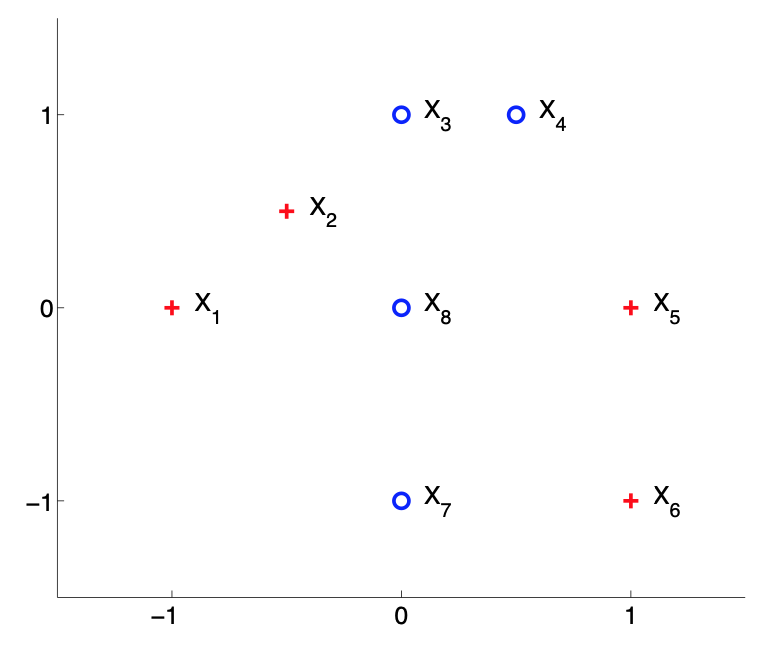
\includegraphics[width =.4 \textwidth]{hw}
\end{center}
%\caption{ A small dataset, for binary classification with AdaBoost.}
\end{figure}
\vspace{-.3in}

\begin{table}[h!]
\begin{center}
\caption{Values of AdaBoost parameters at each timestep.}
\vspace{0.1in}
\begin{tabular}{|c|c|c|c|c|c|c|c|c|c|c|c|}\hline
t & $\epsilon_t$ & $\alpha_t$ & $Z_t$ & $D_t(1)$ & $D_t(2)$ & $D_t(3)$ & $D_t(4)$ & $D_t(5)$ & $D_t(6)$ & $D_t(7)$ & $D_t(8)$ \\\hline
1 & & & & & & & & & & & \\
2 & & & & & & & & & & &\\
3 & & & & & & & & & & & \\\hline
\end{tabular}
\end{center}
\end{table}








\end{enumerate}



\end{document}
